
\begin{figure}[htbp]
\renewcommand{\familydefault}{\sfdefault}\normalfont
\centering 
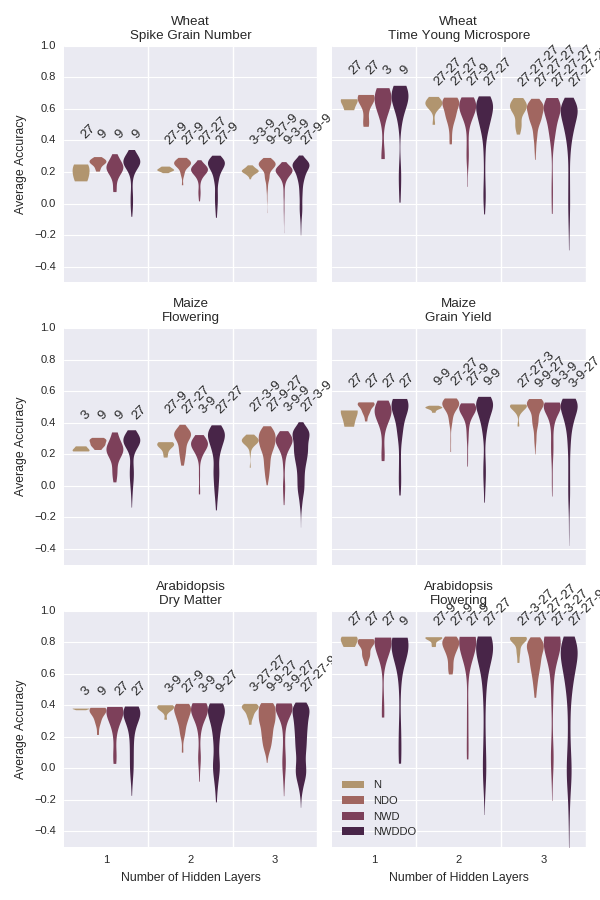
\includegraphics[width=\linewidth]{g3_article/figures/depth_comparison.png}
    \caption{Distribution of predictive accuracy by benchmark dataset, network depth, and model.
             The violin plot width indicates the Kernel Density Estimate (KDE) of all observed 
             accuraies of all models at a given network depth. The number of contributing data points
             to the KDE depends on the number of model hyper parameters evaluated. For model N, there 
             are no hyper parameters. For models NWD and NDO, there are 5, and for model NWDDO, there
             are 25 (5*5). In summary, the KDE plots are constructed from
             $n=hidden*runs*folds*[p1]*[p2] ; n=7*3*10*[5]*[5] ; n=\{ 210, 1050, 7350 \}$ samples. 
             The models contributing to each KDE vary across one or more of their weight decay, dropout, and 
             hidden layer parameters and can be understood as the distribution of results across 
             the set of hyper-parameters to all network models with the same depth and regularization
             type. The KDE bandwidth parameters are set using Scott's normal reference rule. 
             Negative accuraies are the result of trained models producing predictions that 
             are negatively correlated with actual model performance. The KDE plots are 
             trucated to the minimum and maximum observed values in the dataset. The 
             highest mean performing model's shape is listed above each KDE plot as a 
             example of a highly effective network archetecture for that particular dataset, 
             network type, and hidden layer size.} 
\label{fig:depth-comparison}
\end{figure}

